\documentclass[12pt,a4paper]{article}

% --------------------
% Packages
% --------------------
\usepackage[margin=1in]{geometry}
\usepackage{graphicx}
\usepackage{fancyhdr}
\usepackage{setspace}
\usepackage{titlesec}
\usepackage{enumitem}
\usepackage{xcolor}
\usepackage{hyperref}
\usepackage{subcaption}
\usepackage[table]{xcolor}
\usepackage{colortbl}
\usepackage{makecell}
\usepackage{svg}

% --------------------
% Paragraph formatting
% --------------------
\setlength{\parindent}{0pt}  % Remove paragraph indentation
% \setlength{\parskip}{1em}    % Optional: add space between paragraphs

% --------------------
% Project Information
% --------------------
\newcommand{\CompanyName}{Pressure Control Solutions}
\newcommand{\ReportTitle}{Quattroflow Pressure Dynamics}
\newcommand{\ReportSubTitle}{Without and With a Downstream Equilibar in Parallel}
\newcommand{\AuthorName}{Hubald Verzijl}
\newcommand{\AuthorEmail}{hubald@pressurecontrolsolutions.com}
\newcommand{\VersionNumber}{1.0}
\newcommand{\ReportDate}{March 6, 2026}

\hypersetup{
    colorlinks=true,
    linkcolor=blue,
    filecolor=magenta,      
    urlcolor=cyan,
    pdftitle={\ReportTitle},
    pdfauthor={\AuthorName},
    pdfkeywords={Pressure, Dynamics, Quattroflow, Equilibar, Report},
}

% --------------------
% Header & Footer
% --------------------
\pagestyle{fancy}
\fancyhf{} % Clear default header/footer

% Header
\setlength{\headheight}{30pt}
\fancyhead[L]{%
  
\includegraphics[height=0.75cm]{../images/logo.png}
}
\fancyhead[R]{Report Version \VersionNumber}

% Footer
\fancyfoot[C]{\thepage}

\renewcommand{\headrulewidth}{0.4pt}
\renewcommand{\footrulewidth}{0.4pt}

% --------------------
% Title Page
% --------------------
\begin{document}

\begin{titlepage}
    \thispagestyle{fancy}
    \fancyfoot{} % Clear footer for this page only
    \centering
    \vspace*{2cm}
    {\Huge \bfseries \ReportTitle \par}
    \vspace{0.5cm}
    {\Large \ReportSubTitle \par}
    \vspace{2cm}
    \begin{center}
        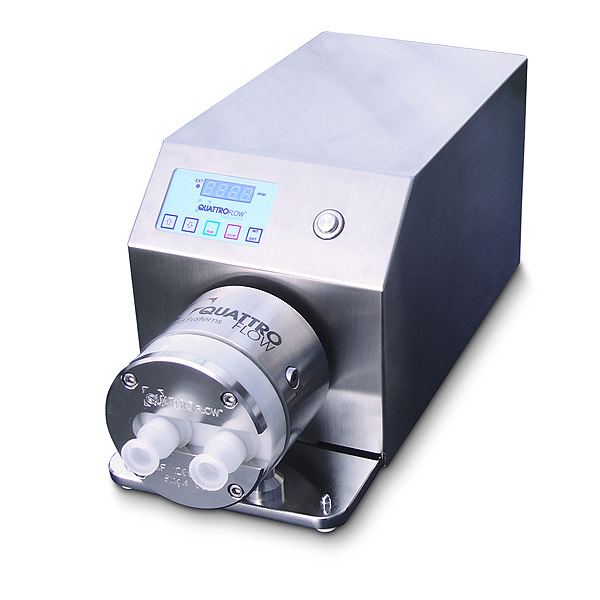
\includegraphics[height=7.5cm]{specific_images/qf1200su-ht.jpg}
    \end{center}
    \vspace{2cm}
    {\Large \CompanyName \par}
    \vspace{0.25cm}
    {\small Author: \AuthorName \par}
    \vspace{0.25cm}
    {\small Report Version: \VersionNumber \par}
    \vspace{0.25cm}
    {\small Date: \ReportDate \par}
    \vfill
\end{titlepage}

% --------------------
% Table of Contents
% --------------------
\section*{Introduction}

This report describes some of the pressure dynamics of a Quattroflow QF150 SU pump. The pump consists of four diaphragm chambers that are sequentially driven by an eccentric shaft. As a result, four pressure pulses are expected per revolution of the pump.

An Equilibar pressure regulator installed downstream of the pump, and in parallel with the process, may be used to reduce pressure fluctuations generated by the pump. In addition, the Equilibar can act as an overpressure relief mechanism, protecting the system from excessive pressures.

In this report, experiments are performed both without and with an Equilibar backpressure regulator circuit activated. The objective is to evaluate the effect of this configuration on the pressure fluctuations generated by the pump.

The results presented in this report provide insight into the potential benefits of using an Equilibar regulator in combination with a Quattroflow pump.

\tableofcontents
\newpage

% --------------------
% Report Content
% --------------------
\section{Sensor validation}
Before performing the actual experiments, both Keller 20SX sensors are validated by connecting them in series and in parallel downstream of the Quattroflow pump, as shown in Figure \ref{fig:serie} and Figure \ref{fig:parallel}. The needle valves resemble the user process resistance.

\begin{figure}[!htbp]
    \centering
    \begin{minipage}{0.45\textwidth}
        \centering
        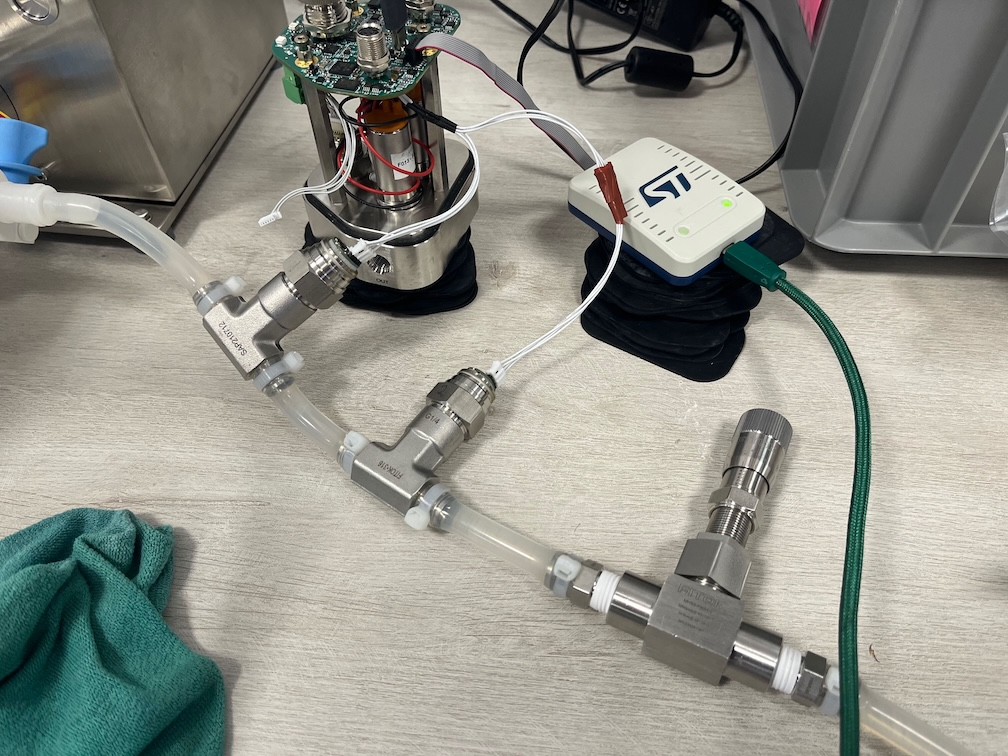
\includegraphics[width=\textwidth]{specific_images/serie.jpeg}
        \caption{Sensors connected in serie for validation test.}
        \label{fig:serie}
    \end{minipage}
    \hfill
    \begin{minipage}{0.45\textwidth}
        \centering
        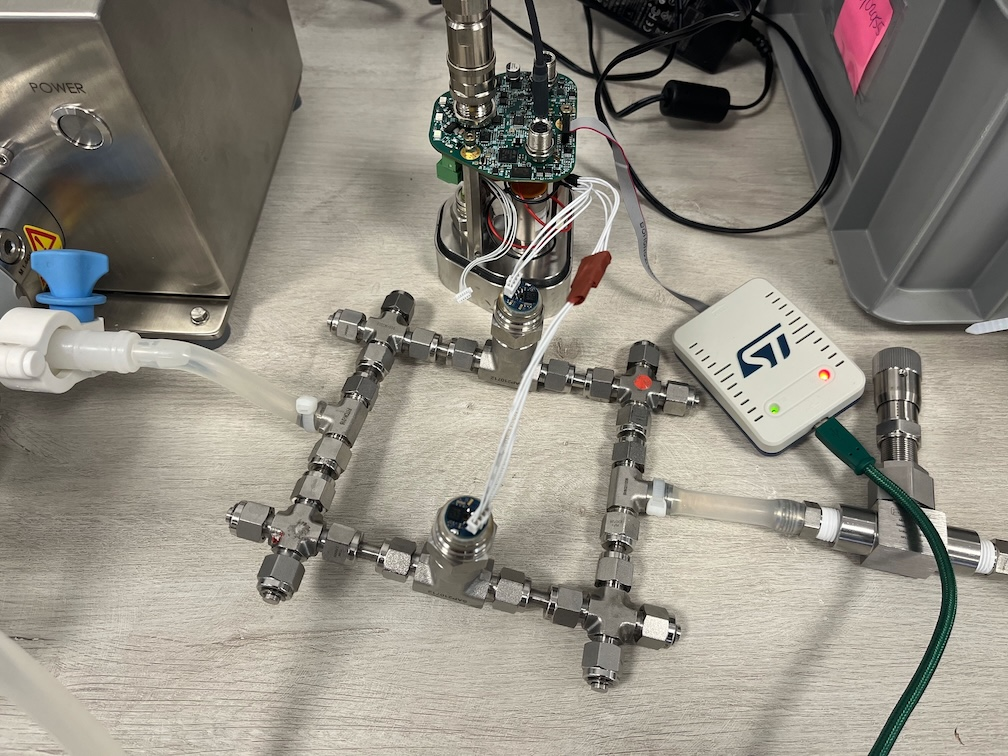
\includegraphics[width=\textwidth]{specific_images/parallel.jpeg}
        \caption{Sensors connected in parallel for validation test.}
        \label{fig:parallel}
    \end{minipage}
    \hfill
\end{figure}

The results of this validation test are shown in Figure \ref{fig:sensor_validation}. From Figure \ref{fig:validation_serie}, it is clear that an increase in RPM while using a needle valve downstream leads to an increase in absolute pressure, as expected. The relative fluctuations are shown in Figure \ref{fig:validation_serie_mean_subtracted}. 

However, the upstream and downstream pressures in the series configuration are not equal, while they are equal in the parallel configuration (Figure \ref{fig:validation_parallel_mean_subtracted}). Although this indicates that the sensors are measuring correctly, it also shows that the fluidic system introduces some oscillatory behavior, especially at higher frequencies. This leads to phase and amplitude differences between both sensors in the series configuration.

\subsection{Conclusion}
\begin{itemize}
    \item The sensors measure identically, as they show similar pressure dynamics in the parallel configuration.
    \item The fluidic system introduces additional dynamics, resulting in phase and amplitude differences between both sensors in the series configuration.
    \item The use of pipes and sensor holders designed specifically for fluids is recommended to reduce the influence of the fluidic system on the pressure dynamics in future experiments.
\end{itemize}

\begin{figure}[htbp!]
    \begin{subfigure}{\linewidth}
        \centering
        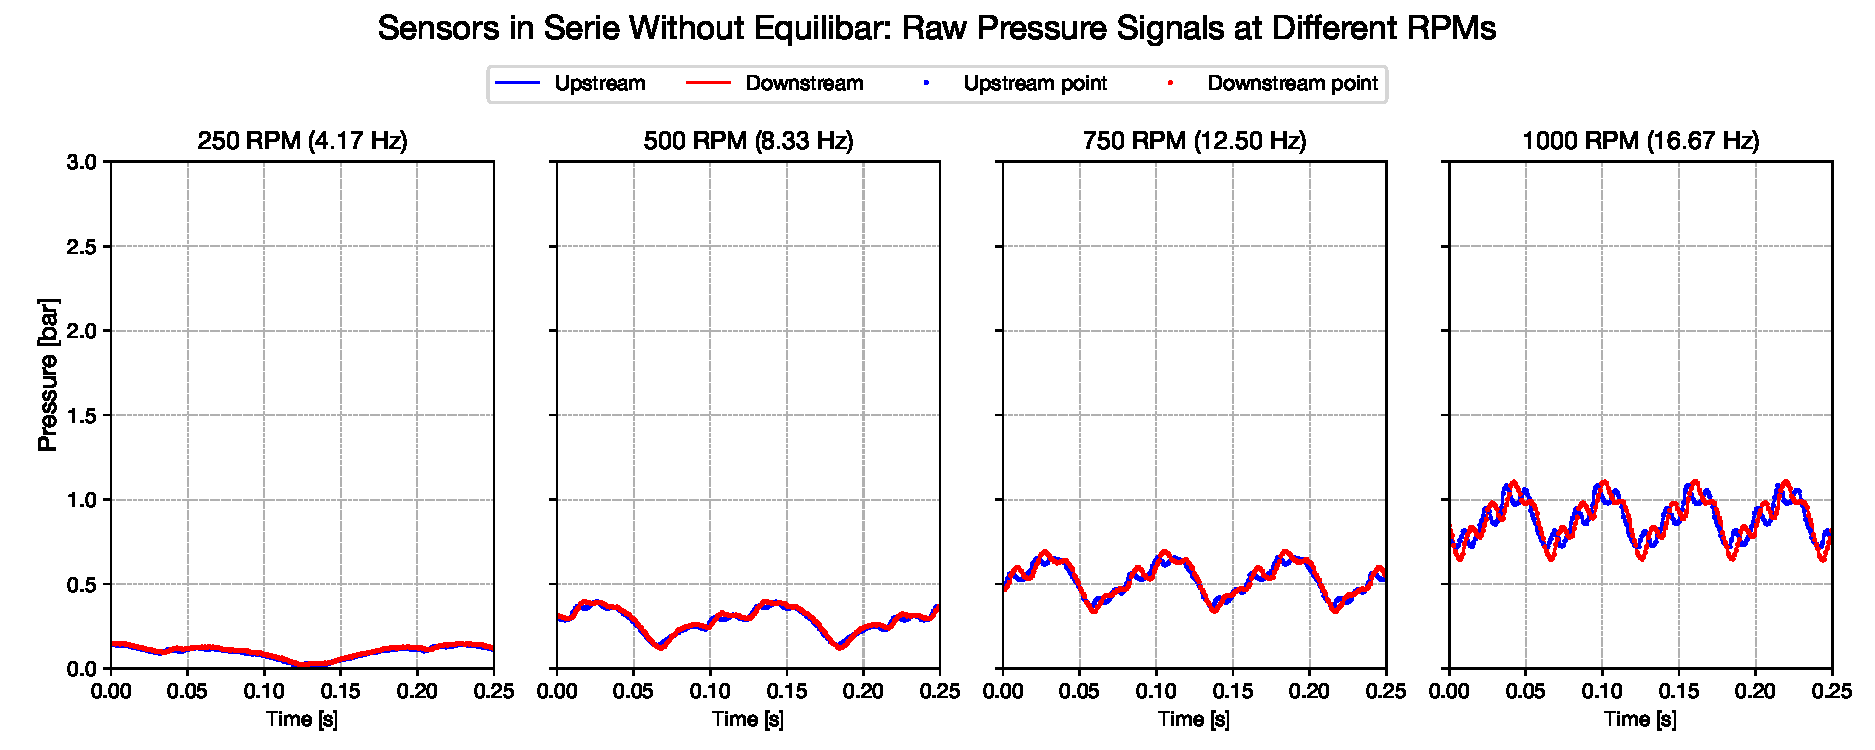
\includegraphics[width=\textwidth]{specific_images/pdf_20260116/2_serie_open.pdf}
        \caption{Sensor validation test with sensors connected in \textbf{serie} (Figure \ref{fig:serie}).}
        \label{fig:validation_serie}
    \end{subfigure}

    \par\bigskip

    \begin{subfigure}{\linewidth}
        \centering
        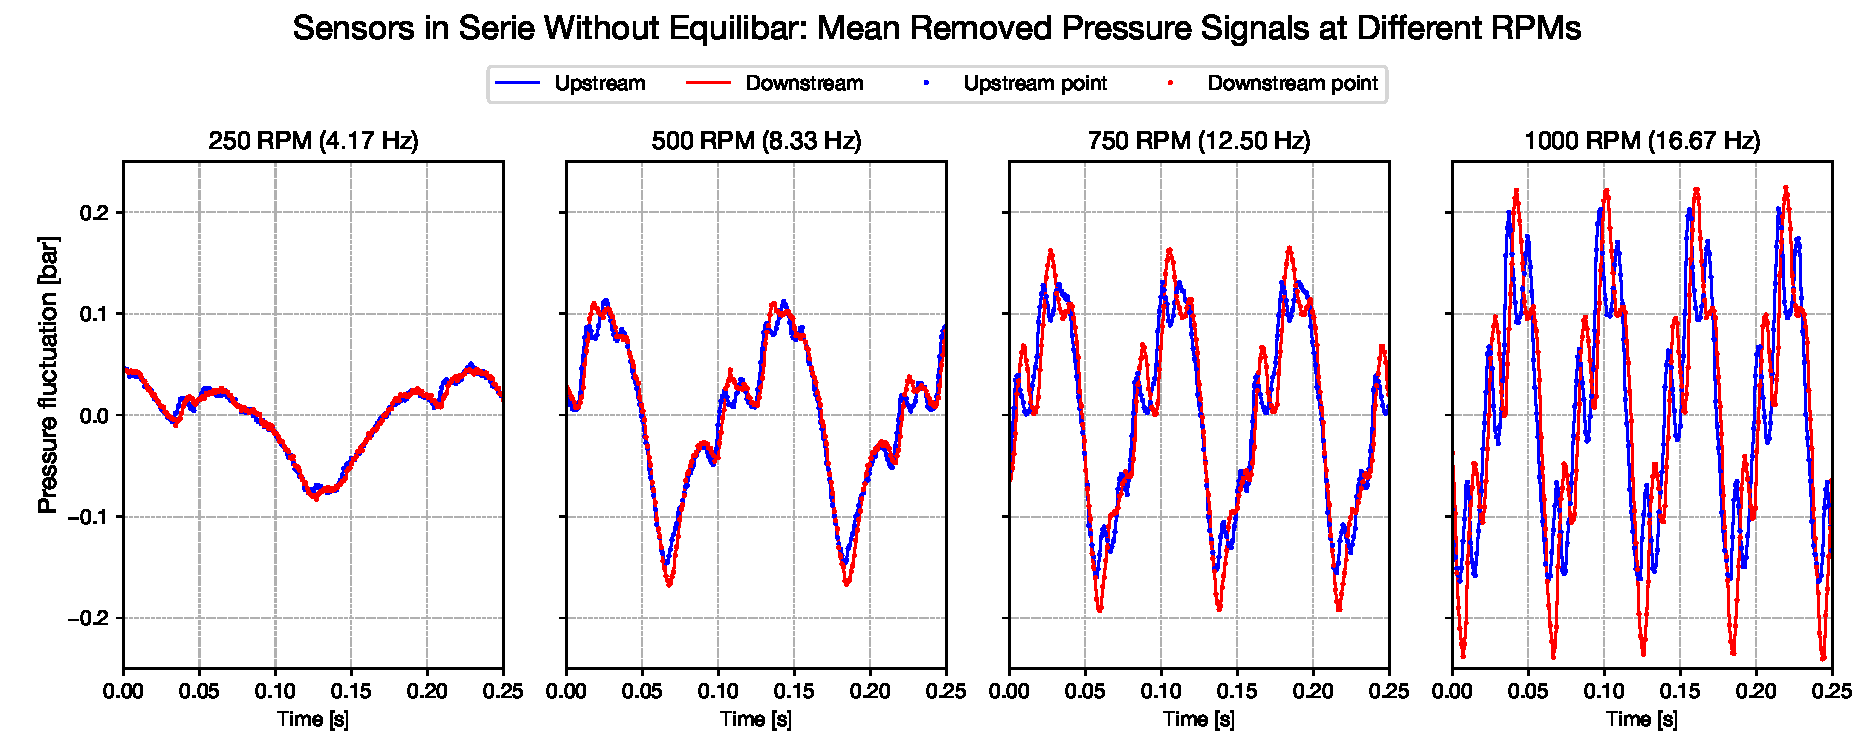
\includegraphics[width=\textwidth]{specific_images/pdf_20260116/2_serie_open_mean_subtracted.pdf}
        \caption{Sensor validation test with sensors connected in \textbf{serie} (Figure \ref{fig:serie}). Pressure fluctuations with average subtracted.}
        \label{fig:validation_serie_mean_subtracted}
    \end{subfigure}

    \par\bigskip

    \begin{subfigure}{\linewidth}
        \centering
        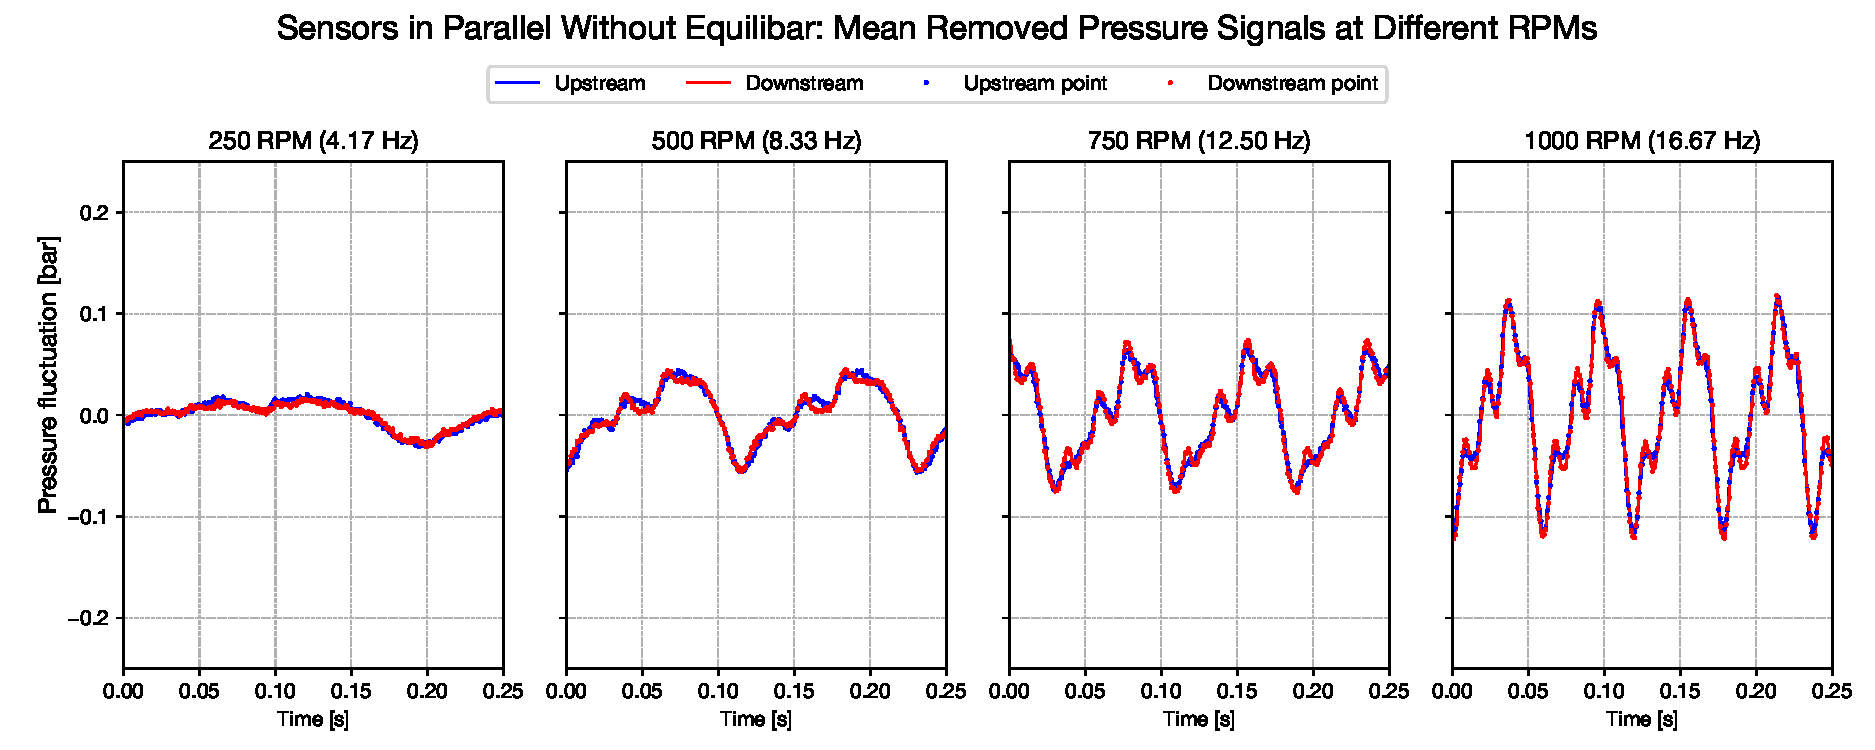
\includegraphics[width=\textwidth]{specific_images/pdf_20260116/1_parallel_open_mean_subtracted.pdf}
        \caption{Sensor validation test with sensors connected in \textbf{parallel} (Figure \ref{fig:parallel}). Pressure fluctuations with average subtracted.}
        \label{fig:validation_parallel_mean_subtracted}
    \end{subfigure}

    \caption{Results of the sensor validation tests. Both sensors show similar pressure dynamics in the \textbf{parallel} case, indicating that they are functioning correctly.}
    \label{fig:sensor_validation}
\end{figure}


\clearpage
\section{Main experiment: Equilibar in parallel}
\subsection{Setup}
A setup is created in which an Equilibar FD Series\footnote{\href{https://www.equilibar.com/PDF/Equilibar-Sanitary_FD_Series-Back_Pressure_Regulators.pdf}{Equilibar FD Series datasheet}} is placed in parallel with the process. This Equilibar incorporates two diaphragms: a control diaphragm and a sealing diaphragm. The reference pressure for the Equilibar is created by an EQ-DA. A ball valve is used to model the process resistance.

\begin{figure}[!htbp]
  \centering
  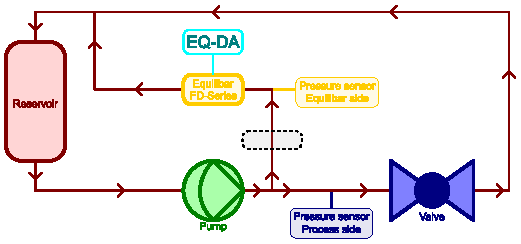
\includegraphics[width=1\textwidth]{specific_images/setup/Setup_1.pdf}
  \caption{Setup with Equilibar in parallel. Reservoir shown in red, Quattroflow pump shown in green, Equilibar orange, EQ-DA in cyan, and pressure sensors shown in orange and blue. The process is modeled by a ball valve shown in blue. In the dotted rectangle pliers can be placed to disable the flow through the Equilibar.}
  \label{fig:setup_parallel}
\end{figure}

\subsection{Hypothesis}
Incorporating an Equilibar FD Series (with two diaphragms) in this setup has two potential advantages:
\begin{itemize}
    \item \textbf{Limiting maximum process pressure:} If the resistance in the process increases, the membrane pump will not lower the RPMs automatically, so the upstream pressure can increase significantly. By placing the Equilibar in parallel, the maximum process pressure can be limited to the applied reference pressure at the Equilibar (due to the control diaphragm), which can potentially protect the system from overpressure.
    \item \textbf{Damping pressure fluctuations:} The Equilibar can potentially dampen (by the sealing diaphragm) the pressure fluctuations generated by the pump, leading to a more stable pressure output. This can be especially beneficial in applications where precise pressure control is required.
\end{itemize}

\subsection{Method}
To demonstrate the second advantage, experiments are performed at 250, 500, 750, and 1000 RPM. During the experiments, the valve is controlled manually such that the upstream process pressure is approximately 1 bar. Each experiment starts with the Equilibar parallel configuration enabled. After some time, pliers are applied to disable the Equilibar circuit.

\subsection{Results}
The results are shown in Figure \ref{fig:parallel_results} and Figure \ref{fig:parallel_rms_vs_rpm}. From these figures, it can be seen that the pressure fluctuations at the process side are often reduced when using the Equilibar in parallel (red versus green areas), especially at lower pump speeds. This indicates that the Equilibar is effective in damping the pressure fluctuations generated by the Quattroflow pump.

To compare these amplitude fluctuations further, Figure \ref{fig:parallel_rms_vs_rpm} shows the RMS of the pressure fluctuations at the process side for both cases (with and without the Equilibar in parallel) at different pump speeds. From this figure, it can be seen that the RMS of the pressure fluctuations is generally lower when using the Equilibar in parallel, particularly at lower pump speeds. These results could potentially be used in marketing materials to illustrate the effect of an Equilibar in parallel on pressure fluctuations.

% INlcude figure
\begin{figure}[!htbp]
    \centering
    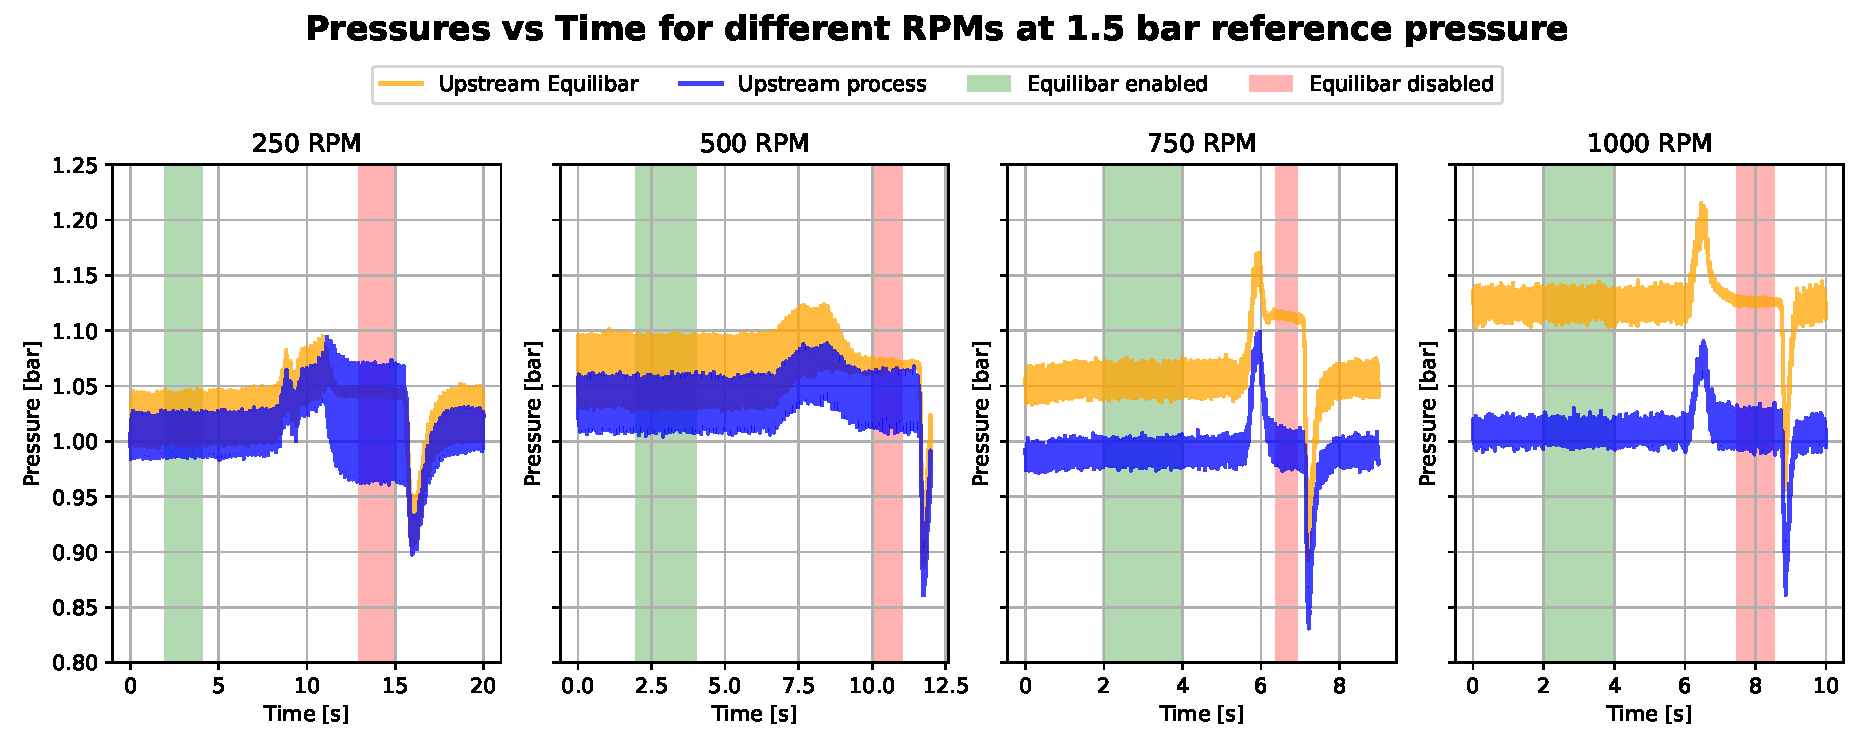
\includegraphics[width=1\textwidth]{specific_images/pdf_20260206/pressure_vs_time_1_5ref.pdf}
    \caption{Pressure dynamics with an Equilibar in parallel at variable backpressures. Pliers are applied in the black rectangle of Figure \ref{fig:setup_parallel}, which corresponds to the red area in the figure. Without pliers, the Equilibar is active, which is illustrated by the green area in this figure. Within the colored areas, the pressure fluctuations upstream of the process are outcome measures.}
    \label{fig:parallel_results}
\end{figure}

\begin{figure}[!htbp]
    \centering
    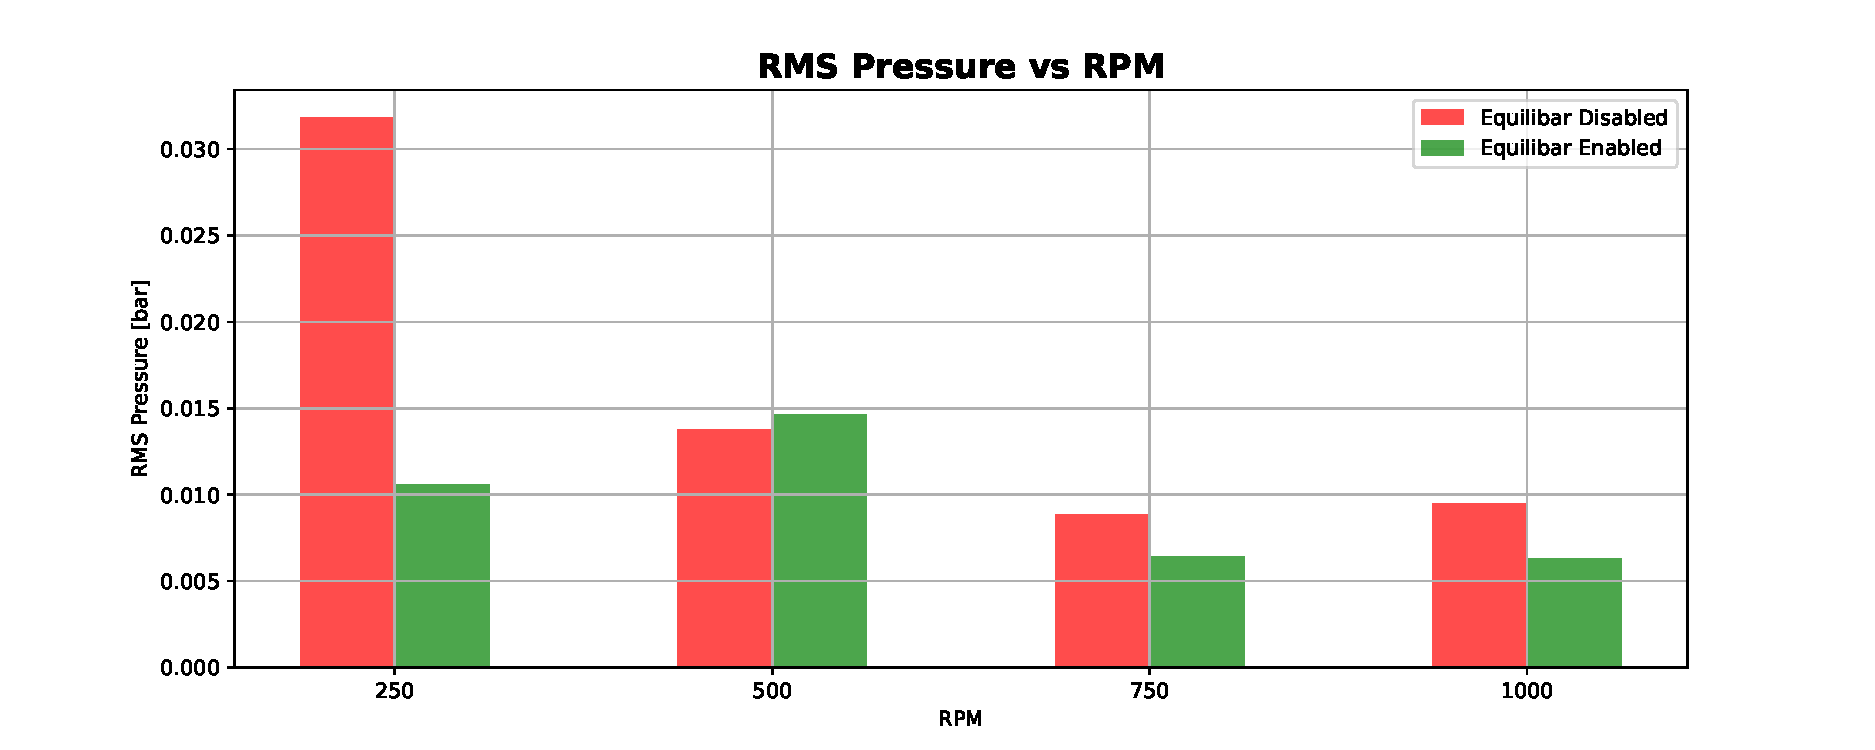
\includegraphics[width=0.8\textwidth]{specific_images/pdf_20260206/rms_pressure_vs_rpm.pdf}
    \caption{Pressure dynamics without and with an Equilibar in parallel at variable backpressures. The bars indicate the RMS of the pressure fluctuations at th upstream process side for both cases at different pump speeds.}
    \label{fig:parallel_rms_vs_rpm}
\end{figure}

\newpage

\subsection{Conclusion}
\begin{itemize}
    \item The Equilibar-in-parallel setup effectively limits the maximum process pressure, thereby protecting the system from overpressure;
    \item In general, the Equilibar-in-parallel setup dampens pressure fluctuations generated by the Quattroflow pump, resulting in a more stable pressure output.
    \item In the investigated setup, at 250 RPM the RMS is \textbf{reduced} by 66.8\%, by 27.9\% at 750 RPM, and by 33.3\% at 1000 RPM. The RMS is \textbf{increased} by 6.3\% at 500 RPM.
    \item The Equilibar-in-parallel setup is not always effective in damping pressure fluctuations, as the RMS of the pressure fluctuations is slightly increased at 500 RPM. This could be due to the specific dynamics of the system at this pump speed, or the fact that the pump generates smaller pressure fluctuations at this speed/specific speeds. Further investigation is needed to understand this behavior.
\end{itemize}


\newpage

\section{Recommendations for further investigation}
\begin{itemize}
    \item Use dedicated tubing designed for fluids to reduce the influence of the fluidic system on the pressure dynamics.
    \item Use different types of diaphragms within the Equilibar to investigate how the Equilibar dynamics influence the pressure damping effect.
    \item Actively reduce fluctuations by closed-loop control of the reference pressure at the Equilibar based on the fluctuating upstream pressure sensor signal. The downstream pressure could also potentially be controlled to maintain an even more constant pressure. The latter could also be used to create a more constant output flow.
    \item Apply an Equilibar in series downstream of the pump. This will compensate for higher pressures upstream of the pump and might also reduce the pressure fluctuations at the process side. However, it is expected that the pressure fluctuations at the pump side will increase, since the Equilibar introduces additional flow resistance in the system, after which the fluctuations may be damped by the Equilibar. A passive Equilibar can be used, but also an active controlled Equilibar to further dampen the fluctuations.
    \item Investigate how a regular resistance (e.g., a needle valve) in series upstream of the process might also dampen some of the oscillations.
\end{itemize}
% --------------------
% References
% --------------------
% \begin{thebibliography}{9}
% \bibitem{ref1}
% Author, \textit{Title of Reference}, Publisher, Year.
% \end{thebibliography}

% Punten
% Fluctuaties upstream of juist downstream verminderen?
% When process pressure is equal to reference pressure, the air in reference pressure acts as an compressible volume, which can dampen fluctuations?

% Vervolgstappen
% Overleg met Bas over huidige resultaten
% Wens: 
% - Flowcontrol zonder stabiele voordruk
% - Stabiele voordruk met continue afblazen? Of juist met actieve regeling?
% 13 februari naar PCS?

% 6 februari 
% Scan through all different resistances for variable frequencies


\end{document}
